% Four additional figures, drawn 2026-11-11 from recorded data by
% mimic-video-repro/eval/analysis/render_paper_figures_extra.py.
% This file is NOT \input by main.tex. Since 2026-11-11 the four figures are in the supplement
% (sec/X_suppl.tex, labels fig:supp_*). The environments below are the main-text versions: when you
% move one into the paper, delete its copy in the supplement.
% Every number in the captions is in mimic-video-repro/figures/paper/figure_numbers_extra.json.

% ---------------------------------------------------------------------------------------------
% (1) Accuracy versus cost. Parsed from tables/main_results.tex, so re-render after editing Table 1.
%     Two-column version below; the one-column cut (latency only) is fig7_cost_accuracy_1col.pdf.
\begin{figure*}[t]
  \centering
  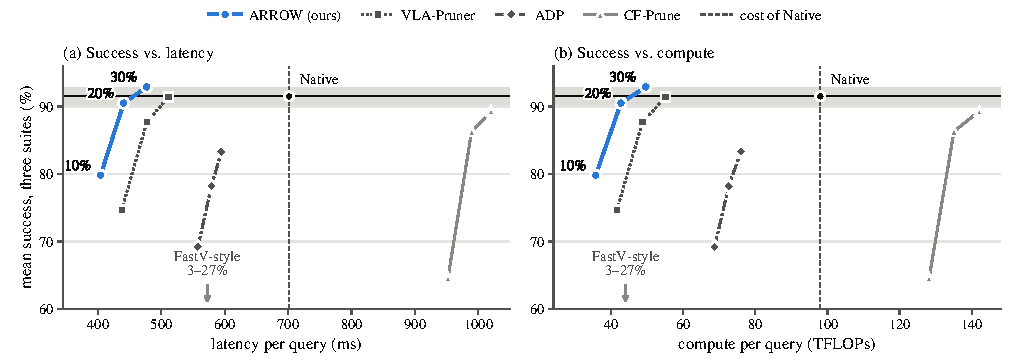
\includegraphics[width=\linewidth]{fig7_cost_accuracy.pdf}
  \caption{\textbf{Success versus inference cost on mimic-video.}
  Each line joins the 10\%, 20\% and 30\% settings of one method in \cref{tab:main_mimic}; success is the mean over the three LIBERO suites.
  Costs include every dense call and probe a method makes.
  The black line and grey band show Native with its Wilson 95\% confidence interval over 1,500 episodes, and the dashed line marks its cost.
  FastV-style lies below the plotted range.}
  \label{fig:cost_accuracy}
\end{figure*}

% ---------------------------------------------------------------------------------------------
% (2) Router scores versus task-agnostic criteria (offline, LIBERO-Spatial). One column.
\begin{figure}[t]
  \centering
  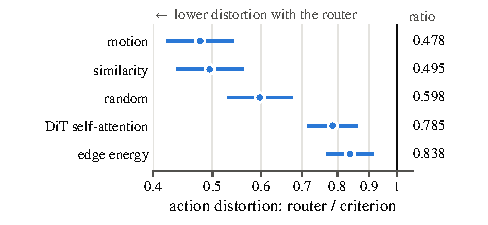
\includegraphics[width=\linewidth]{fig8_criteria_forest.pdf}
  \caption{\textbf{Router scores versus task-agnostic criteria.}
  Ratio of offline action distortion when the same spatial coarsening follows router scores instead of each criterion, on 50 held-out LIBERO-Spatial episodes (200 windows).
  Points are geometric means and bars are 95\% confidence intervals; values below one mean lower distortion with the router.}
  \label{fig:criteria_forest}
\end{figure}

% ---------------------------------------------------------------------------------------------
% (3) Allocation on real queries of five tasks per suite. Two columns.
%     fig9_allocation_gallery_full.pdf archives all ten candidates per suite; it is not included.
\begin{figure*}[t]
  \centering
  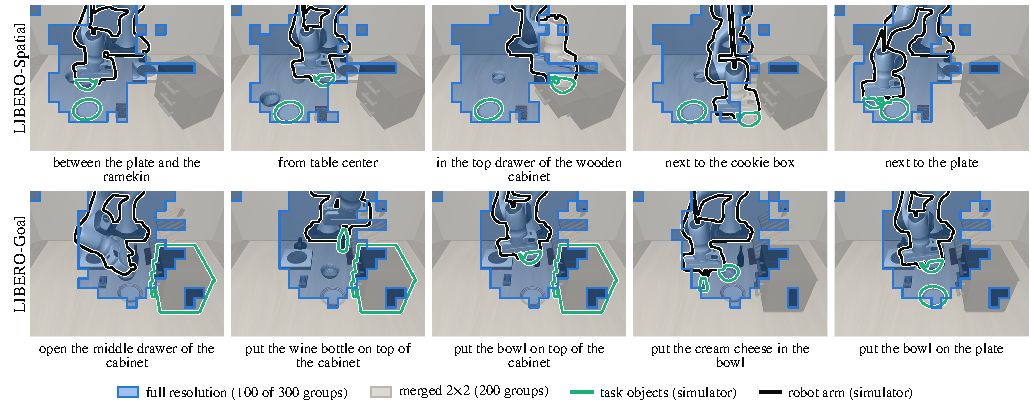
\includegraphics[width=\linewidth]{fig9_allocation_gallery.pdf}
  \caption{\textbf{Full-resolution groups across tasks.}
  Five tasks from each of LIBERO-Spatial, LIBERO-Object and LIBERO-Goal at the 20\% future-token budget, selected for the highest mean coverage of task-object and robot-arm pixels by full-resolution groups.
  Each panel uses the first recorded episode and the query nearest 12.
  Blue marks the 100 groups kept at full resolution and grey the 200 merged groups; outlines are simulator masks of task objects (green) and the robot arm (black).
  Spatial labels give the location of the bowl to pick up.
  These selected examples illustrate spatial overlap; they do not estimate average coverage.}
  \label{fig:allocation_gallery}
\end{figure*}

% ---------------------------------------------------------------------------------------------
% (4) Latency by stage. One column.
\begin{figure}[t]
  \centering
  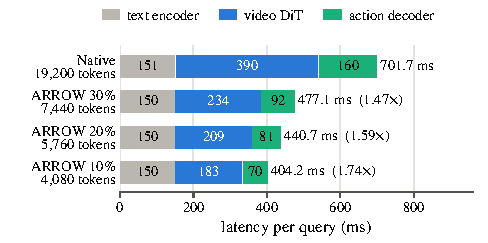
\includegraphics[width=\linewidth]{fig10_latency_breakdown.pdf}
  \caption{\textbf{Where the time of one query goes.}
  Median stage times on an H100 at batch size one, with CUDA graphs for both policies.
  Text encoding takes about 150\,ms in every setting.
  At the 20\% budget the video DiT runs $1.87\times$ and the action decoder $1.98\times$ faster than in Native, which gives $1.59\times$ end to end while total FLOPs fall by 56\%.
  Totals are the medians over 32 calls reported in \cref{tab:main_mimic}; stage times are medians over five traced calls.}
  \label{fig:latency_breakdown}
\end{figure}
